\newpage
\section{RPL}\label{sec:state-rpl}
\renewcommand{\rightmark}{RPL}
%TODO tour des protocoles de routages ??

Routing Protocol for Low-Power and Lossy Networks (RPL) est un protocole de routage IPv6 destiné aux réseaux dont les noeuds sont contraints en énergie et dont les liens entre ces noeuds sont soumis à des pertes importantes de paquets (Low-power and Lossy Networks (LLNs)).
Ce protocole à vecteur de distance est un protocole proactif, c'est à dire que les routes sont établies avant qu'elles ne soient nécessaires.

RPL sépare le traitement et la transmission des paquets de l'optimisation de l'objectif de routage. Cela permet de l'adapter à un large éventail d'applications des LLNs.

\subsection*{Topologie}
%TODO exemple de topologie + collect application noeuds-> racine
La topologie utilisée par RPL et le DODAG (Destination Oriented Dag). Un DODAG est un graphe dirigé acyclique (DAG) ayant une seule racine.
\begin{figure}[H]
    \centering
    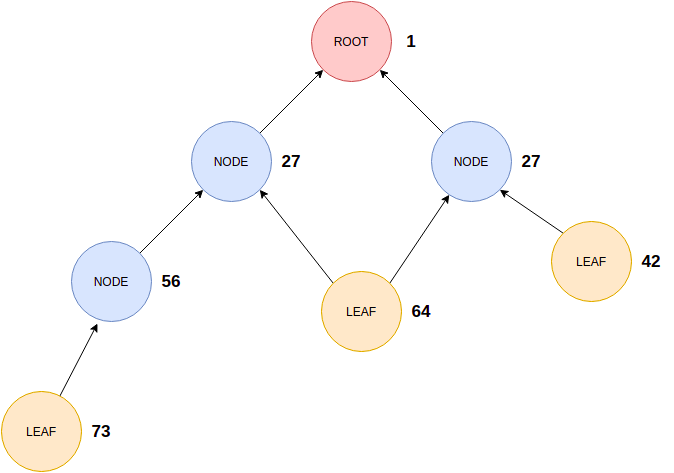
\includegraphics[scale=0.45]{res/dodag.drawio.png}
    \caption{DODAG.}
    \label{fig:state-dodag}
\end{figure}


\subsection*{Fonctions objectif}
%TODO expliquer brievement MRHOF et 0F0 (celles implémentées dans contiki)
Une fonction objectif (OF) défini comment plusieurs métriques sont utilisées pour calculer le rang d'un noeud. Le rang d'un noeud détermine sa position dans le DODAG par rapport aux autres noeuds.
Le rang augmente stictement dans le sens descendant et diminue strictement dans le sens montant. Ainsi, $rang(n)>rang(parent(n))$. La figure~\ref{fig:state-dodag} illustre un DODAG avec des valeurs de rang fictives attribuées aux noeuds. Sur cet exemple, la racine du DODAG a comme range, la valeur par défaut \textsc{root\_rank} définie dans le RFC.

Cette section décris brièvement deux fonctions objectif implémentées dans Contiki: OF0 et MRHOF.
\begin{itemize}
    \item \subsubsection*{OF0}%rfc6552
            Objective Function Zero est une fonction dont l'objectif est de choisir un parent qui permettra à un noeud d'avoir la racine du DODAG le plus proche possible. Le rang d'un noeud $R(N)$ est calculé comme suit:
            \begin{equation}
                ranck\_increase = (Rf * Sp + Sr) * MinHopRankIncrease
                \newline
                R(N) = R(P) + ranck\_increase
            \end{equation}
    \item \subsubsection*{MRHOF}
            Minimum Rank with Hysteresis Objective Function
\end{itemize}




\subsection*{Types de messages}
%TODO décrire le format des différents messages

\subsection*{Construction du réseau}
%TODO décrire les étapes de construction d'un réseau

\subsection*{Modes de fonctionnements}
%TODO parler des différents modes de fonctionnement: Storing mode/non-storing mode

\subsection*{Discussion}
%TODO RPL good parce que fait pour LLN (intro article eval RPL) et implémenté dans Contiki mais améliorations pour l'exterieur et grands réseaux (conclusion article eval RPL)
%%bib:
%@INPROCEEDINGS{5464820,
%  author={Tripathi, J. and de Oliveira, J. C. and Vasseur, J. P.},
%  booktitle={2010 44th Annual Conference on Information Sciences and Systems (CISS)}, 
%  title={A performance evaluation study of RPL: Routing Protocol for Low power and Lossy Networks}, 
%  year={2010},
%  volume={},
%  number={},
%  pages={1-6},
%  doi={10.1109/CISS.2010.5464820}}